\chapter{Wake-Up}

Molto spesso, in un ambiente distribuito, ci troviamo di fronte alla seguente
situazione:\\
Deve essere svolto un compito in cui devono essere coinvolte tutte le entità;
tuttavia solo alcune di esse sono indipendentemente \textbf{attive} (a causa di
un evento spontaneo, o per aver terminato un calcolo precedente) e pronte per il
calcolo, le altre sono \textbf{inattive}, nemmeno consapevoli del calcolo che
deve avvenire. \\
In queste situazioni, per eseguire il compito, dobbiamo assicurarci che tutte le
entità diventino attive. Chiaramente, questo passaggio preliminare può essere
avviato solo dalle entità già attive; tuttavia, non sanno quali altre entità (se
presenti) sono già attive.\\
Questo problema è chiamato \textbf{Wake-up}: un'entità attiva è solitamente
chiamata \textbf{awake}, un'entità inattiva (ancora) è chiamata \textbf{asleep};
il compito è svegliare tutte le entità.\\
Non è difficile vedere la relazione tra il broadcasting e il wake-up: \textbf{il
    Broadcasting è un wake-up con una sola entità inizialmente sveglia; al
    contrario, il wake-up è un broadcasting con possibilmente molti iniziatori}
(cioè, inizialmente più di un'entità ha le informazioni). In altre parole,
\textbf{il broadcasting è solo un caso speciale del problema del wake-up}.\\
È interessante, ma non sorprendente, che la strategia di flooding utilizzata per
il broadcasting risolva effettivamente il problema più generale del wake-up. Il
protocollo modificato è chiamato WFlood. Inizialmente tutte le entità sono
\textit{asleep}; qualsiasi entità \textit{asleep} può svegliarsi (diventare
\textit{awake}) spontaneamente e avviare il protocollo.\\
Non è difficile verificare che il protocollo termini correttamente con le
restrizioni standard. \vspace{1cm}\\

\section{Protocollo WFlood}
\textbf{Problema}: Il problema del wake-up consiste nell'avere una
configurazione iniziale del nostro sistema in cui possono essere presenti più
entità sveglie (in stato di AWAKE) al tempo $t=0$ (ovvero più iniziatori) e le
restanti entità saranno dormienti (ASLEEP). Al termine del protocollo vogliamo
che tutte le entità siano sveglie (AWAKE). Utilizzeremo sempre l'idea del
Flooding, ovvero un'entità invia l'informazione a tutti i suoi vicini tranne
quello che gliel'ha inviata. Formalmente:

$$
    P_{INIT} =<\; \forall x \in \xi, STATUS(x) = ASLEEP \;>
$$

$$
    P_{FINAL} =<\; \forall x \in \xi, STATUS(x) = AWAKE \;>
$$

\begin{lstlisting} [caption={\textit{Protocollo WFlood.}}]
S = {AWAKE, ASLEEP}
$S_{INIT} = S_{START}$ = {ASLEEP}
$S_{TERM}$ = $S_{FINAL}$ = {AWAKE}

Restrictions = R

ASLEEP
    Spontaneously
    begin 
        send(W) to N(x)
        become AWAKE
    end

    Receiving(W)
    begin
        become AWAKE
        send(W) to N(x) - sender
    end
\end{lstlisting}

\textbf{Descrizione del protocollo (codice)}: $P_{init}$ ci dice che tutte le
entità all'inizio si trovano sullo stesso stato, che è quello di Asleep.
Successivamente verranno svegliate (e quindi cambieranno stato) in base agli
impulsi spontanei che ricevono e quello sarà il numero degli iniziatori. Quando
ricevono questo impulso spontaneo inviano l'informazione a tutti i vicini e
cambiano stato in "AWAKE". Quando un'entità nello stato di ASLEEP riceve il
messaggio allora diventa AWAKE e lo invia a tutti i suoi vicini meno il sender.
In poche parole, solamente gli iniziatori lo inviano a tutti, i restanti lo
inviano a tutti meno il sender.

\subsection{Complessità del problema}
\underline{Messaggi:}
Il numero di messaggi è almeno pari a quello del broadcast; in realtà, non è
molto di più. E questo avviene quando c'è un solo iniziatore come nel Broadcast
e quindi tutte le entità meno una riescono a risparmiare messaggi.

\begin{itemize}
    \item \textit{Caso Migliore} $(\Omega)$: $M[$\texttt{WFlood}$] \geq 2m - n +
              1$
    \item \textit{Caso Peggiore} $(O)$: $M[$\texttt{WFlood}$] \leq 2m$
    \item \textit{Caso generico con $k^*$ iniziatori}: $2m-n+1 + k^* -1 =
              2m-n+k^*$ Dove il $-1$ è l'iniziatore già incluso in $2m-n+1$

          $M[$\texttt{Wake-Up}$/R] \geq M[$\texttt{Broadcast}$/RI+] =
              \Omega(m)$\\
          \texttt{WFlood} è ottimo per i messaggi.
\end{itemize}

Il caso peggiore accade quando tutte le entità si svegliano con l'impulso
spontaneo ($n$ initiator).

\subsubsection{Dimostrazione del Lower Bound pari ad m}
Sia A un algoritmo che permette di risolvere il problema del Wake-up con un
numero di messaggi minori di M. Questo significa che se applicassimo A su un
generico grafo G allora ci sarebbe almeno un arco nel quale non vengono
scambiati messaggi. Supponiamo che sia proprio l'arco tra $x$ ed $y$ denominato
$e$. Andiamo adesso a costruire un nuovo grafo, chiamato $G'$ ottenuto
rimuovendo l'arco $e$ tra x ed y e spostando le sue porte tra i nodi $x$ e $z$ e
$y$ e $z$. A per essere un algoritmo che risolve il problema in oggetto deve
dare soluzione su tutte le esecuzioni ed indipendentemente dalla configurazione
iniziale. Vogliamo quindi dimostrare che esiste almeno un esecuzione di A tale
per cui l'algoritmo fallisce. Andiamo quindi ad applicare la stessa identica
esecuzione del protocollo A che aveva su G in G' ovvero:
\begin{itemize}
    \item Tutti gli iniziatori che abbiamo avuto su G li ritroviamo su G', su G
          $z$ nemmeno era presente quindi non può essere iniziatore.
    \item Tutti i tempi ed i ritardi di comunicazione che abbiamo osservato su G
          li riportiamo su G', ovvero che se un messaggio inviato ad un generico nodo ci
          metteva 30 secondi ad arrivare in G allora ci mette 30 secondi anche su G'.
    \item Possiamo eseguire la stessa esecuzione di A perché in G l'arco in cui
          non transitavano messaggi è proprio $e$ ed in G' $e$ nemmeno è presente quindi
          sicuramente non verranno scambiati messaggi su quell'arco
    \item in poche parole forziamo la stessa identica esecuzione su G'.
\end{itemize}
Dato che in quella specifica esecuzione $x$ ed $y$ non inviavano messaggi sulle
porta dell'arco $e$, in questo caso non invieranno i messaggi al nodo $z$.
Quindi quando il protocollo termina tutti i nodi avranno raggiunto uno stato
terminale, tranne $z$ che è ancora in stato di Asleep. Abbiamo quindi
individuato un esecuzione in cui l'algoritmo A fallisce. Se fallisce per UN
esecuzione non possiamo dire che l'algoritmo da soluzione al problema, e quindi
si contraddice l'ipotesi.\\

Il tempo ideale sarà, in generale, più piccolo di quello per il broadcasting:\\
\underline{Tempo:}
\begin{center}
    T[$\texttt{Broadcast}/RI+] \geq T[\texttt{Wake-Up}/R] = \Omega(d)$\\
    $T[\texttt{WFlood}] = \Theta(d)$\\
\end{center}
\texttt{WFlood} è ottimo per il tempo (con più initiator si fa prima).\\

Tuttavia, nel caso di un unico iniziatore, i due casi coincidono. Poiché i
limiti superiore e inferiore coincidono in ordine di grandezza, possiamo
concludere che il protocollo WFlood è ottimale sia per numero di messaggi che in
termini di tempo.\\
La complessità di Wake-Up è riassunta dalle seguenti due proprietà,
\begin{itemize}
    \item \textbf{La complessità dei messaggi del Wake-up sotto R è $\Theta(m)$}
    \item \textbf{La complessità del tempo del Wake-up sotto R è $\Theta(d)$}\\
\end{itemize}

\section{WFlood su grafi particolari}
\subsection{Alberi}
Il costo dell'utilizzo del protocollo WFlood per il wake-up dipenderà dal numero
di iniziatori. Infatti, se c'è un solo iniziatore, allora questo è solo un
broadcast e costa solo $n - 1$ messaggi ($m=n-1$). Al contrario, se ogni entità
inizia indipendentemente, ci saranno un totale di $2(n - 1)$ messaggi. Quindi:
\begin{center}
    Caso peggiore:$M[$\texttt{WFlood}$/R] \leq 2(n-1)$ \\
    (tutti sono iniziatori quindi essendo $m = n-1$ abbiamo $2 n-2$)
\end{center}
Supponiamo di avere $k^*$ iniziatori con $k^* \leq n$:
\begin{center}
    $M[$\texttt{WFlood}$/R;T]= 2(n-1) - (n-k^*) = n+k^*-2$\\
    \begin{itemize}
        \item $2(n-1)$ è il caso peggiore a cui vanno tolti:
        \item $(n-k^*)$ Tutte le entità non iniziatrici.
    \end{itemize}
\end{center}

\subsection{Ipercubi}
Nelle precedenti sezioni abbiamo trovato un modo per far scendere il costo del
Broadcast su ipercubi da $O(nlogn)$ a $O(n)$. Nel caso del Wake-up però non è
possibile abbassare il costo, poiché essendoci più iniziatori non vale la regola
del mandare il messaggio a tutte le etichette minori di quella in cui un'entità
ha ricevuto un messaggio. Quindi:
\begin{center}
    $M[$\texttt{Wake-Up}$/R;H_k] = \Omega(n \log n)$ \\
\end{center}
Deve transitare almeno un messaggio per arco, ed essendo il costo anche $O(n
    \log n)$ siamo ottimi.\\
%Diversamente dal problema del \texttt{Broadcast}, qui non possiamo utilizzare
%l'\texttt{HyperFlood} in quanto possiamo avere più initiator.\\
Il tempo quindi rimane lo stesso.
\begin{center}
    $T[$\texttt{WFlood}$/R;H_k] \leq d = k = \log n$ \\
\end{center}
Dove $k$ è l'eccentricità di un nodo all'interno dell'ipercubo

\subsection{Grafi completi}
Tramite l'utilizzo del generico protocollo WFlood il costo sarà il seguente:
\begin{center}
    Caso Peggiore: $M[$\texttt{WFlood}$/R] = O(m) = O(n^2)$ \\
    Caso Migliore: $M[$\texttt{Wake-Up}$/R;k] = \Omega(n^2)$
\end{center}
Utilizzando il protocollo del KBcast e se si svegliassero $k^*$ entità il costo
sarebbe $k^*(n-1)$, ma nel caso peggiore $k^*$ è proprio $n$ quindi il caso
peggiore sarebbe comunque O($n^2$).
\begin{center}
    $M[$\texttt{KBcast}$/R] = k^*(n-1) = O(n^2)$
\end{center}
Questo perché ogni $k^*$ iniziatore invia un messaggio a tutto il suo vicinato
che è $n-1$. Però $1\leq K^* \leq n$ quindi il bound resta comunque O($n^2)$

Quindi con il \texttt{WFlood} siamo ottimi, anche se il costo è alto e non è
possibile usare il \texttt{KBcast} visto nel problema del \texttt{Broadcast} su
grafi completi in quanto non si ottengono migliorie di nessun tipo.

\subsection{Grafi completi con identificatori}
Dato che non si riesce a diminuire il costo del protocollo tramite l'utilizzo
del KBcast, andiamo ad aumentare il numero di restrizioni all'insieme R.
Aggiungiamo quindi la restrizione \textbf{Restriction Initial Distinct Values
    (ID)}: ogni nodo adesso ha associato un identificatore unico che lo distingue
dagli altri. In questo caso possiamo creare un protocollo, che chiameremo
\texttt{WFlood+} con il seguente costo:
%\begin{center} $M[$\texttt{WFlood+}$/R;K_n;id] = O(n \log n)$ \end{center}

\begin{theorem}
    $M[$\texttt{WFlood+}$/R;K;ID] \geq 0.5n \log n$
\end{theorem}

%\textbf{Lemma:} Il numero di messaggi nel problema del WAKE-UP sotto le
%restrizioni di grafo completo e identificatore unico è $\frac{1}{2} n \log n$
Possiamo dimostrare che siamo ottimi, ovvero che siamo anche $O(n \log n)$
tramite la tecnica dell'avversario.

\subsubsection{Tecnica dell'avversario}
Per costruire il peggior scenario possibile per un protocollo A di Wake-up,
consideriamo un gioco tra le entità ed un avversario. Le entità devono obbedire
alle regole del protocollo, mentre l'avversario cercherà di creare lo scenario
peggiore possibile, forzando le entità ad inviare il maggior numero di messaggi.

\paragraph{Assunzioni:} assumiamo che $n$ sia una potenza di due: $n = 2^p$, ovvero
che le entità che si svegliano sono una potenza di due.

\paragraph{Poteri dell'avversario: [SIAMO SU GRAFO COMPLETO]}
\begin{enumerate}
    \item Decide i valori iniziali delle entità (id), purché siano tutti distinti;
    \item Decide quale entità spontaneamente inizia l'esecuzione di A e quando;
    \item Decide quando un messaggio spedito arriva (in tempo comunque finito);
    \item Decide il matching tra gli archi e le etichette (porte). Durante
          l'esecuzione, quando $x$ effettua l'operazione "Invia messaggio alla porta
          $l$" ed $l$ non è stata ancora assegnata, l'avversario sceglierà su quale
          collegamento non ancora utilizzato (ovvero che non sono stati ancora inviati
          messaggi) assegnare porta $l$.
\end{enumerate}

L'invio di un messaggio a più di una porta verrà trattato come l'invio del
messaggio a ciascuna di tali porte una alla volta (in un ordine arbitrario).\\
Qualunque cosa decida l'avversario, può accadere in una vera esecuzione. Vediamo
quanto male può creare un caso l'avversario per A.\\
Due insiemi di entità si diranno \textbf{connessi all'istante $t$} se almeno un
messaggio è stato trasmesso da un'entità di un insieme a un'entità dell'altro.

\textbf{Sviluppo del peggior scenario possibile:}
\begin{enumerate}
    \item Inizialmente l'avversario sveglia una sola entità s, che chiameremo
          Seed, che inizierà l'esecuzione del protocollo. Quando s decide di
          inviare un messaggio ad una certa porta l, l'avversario sveglierà
          un'altra entità $y$ e assegnerà porta l all'arco tra s e y.
          Successivamente ritarda la trasmissione del messaggio fin quando $y$
          non decide di inviare un messaggio ad un'altra porta $l'$;
          l'avversario assegnerà porta $l'$ al collegamento tra $y$ ed $s$ e
          farà in modo che i due messaggi inviati arrivino contemporaneamente.
          In questo modo ogni messaggio raggiungerà un nodo già sveglio e le due
          entità saranno connesse.\\
          D'ora in poi, l'avversario agirà in modo simile; assicurarsi sempre
          che i messaggi vengano inviati ai nodi già attivi e che l'insieme di
          nodi attivi sia connesso.
    \item Si consideri un'entità $x$ che esegue un'operazione di \textbf{invio}
          a un'etichetta non assegnata $a$.
          \begin{enumerate}
              \item Se $x$ ha un collegamento inutilizzato (cioè un collegamento
                    su cui finora non sono stati inviati messaggi) che lo
                    collega a un nodo attivo, l'avversario assegnerà $a$ a quel
                    collegamento.\\
                    In altre parole, l'avversario cercherà sempre di fare in
                    modo che le entità sveglie inviino messaggi ad altre entità
                    sveglie.
              \item Se sono stati utilizzati tutti i collegamenti tra $x$ e i
                    nodi svegli, l'avversario creerà un altro insieme di nodi
                    svegli e collegherà i due insiemi.
                    \begin{enumerate}
                        \item Siano $x_0 , . . . , x_{k-1}$ i nodi attualmente
                              attivi, ordinati in base al loro tempo di
                              risveglio (quindi, $x_0 = s$ è il seed e $x_1 =
                                  y$). L'avversario eseguirà la seguente funzione:
                              scegliere $k$ nodi inattivi $z_0 , . . . ,
                                  z_{k-1}$ ; stabilire una corrispondenza logica tra
                              $x_j e z_j$ ; assegnare i valori iniziali alle
                              nuove entità in modo che l'ordine tra esse sia
                              uguale a quello tra i valori delle entità
                              corrispondenti; svegliare queste entità e
                              costringerle ad avere la "\textbf{stessa}"
                              esecuzione (stessa programmazione e stessi
                              ritardi) come già avevano le corrispondenti.
                              (Quindi, $z_0$ verrà svegliato per primo, il suo
                              primo messaggio verrà inviato a $z_1$ , che verrà
                              svegliato successivamente e invierà un messaggio a
                              $z_0$ , e così via)
                        \item L'avversario assegnerà quindi l'etichetta $a$ al
                              collegamento che collega $x$ alla sua
                              corrispondente entità $z$ nel nuovo set; il
                              messaggio verrà tenuto in transito fino a quando
                              $z$ (come ha fatto $x$) dovrà trasmettere un
                              messaggio su un collegamento inutilizzato
                              (diciamo, con etichetta $b$) ma tutti i bordi che
                              lo collegano al suo insieme di entità sveglie sono
                              già stati utilizzati.
                        \item Quando ciò accade, l'avversario assegnerà
                              l'etichetta $b$ al collegamento da $z$ a $x$ e
                              farà arrivare ed elaborare i due messaggi tra $x$
                              e $z$.
                    \end{enumerate}
                    In altre parole, questo punto può essere descritto come
                    segue:\\
                    Se tutti i link tra un'entità $x$ ed un altro nodo sveglio
                    sono tutti stati utilizzati ed $x$ vuole inviare un
                    messaggio ad una nuova porta, allora l'avversario creerà un
                    altro set di nodi (già svegli) e li forzerà ad avere la
                    stessa esecuzione del set su cui si è basato. Dato che
                    eseguono la stessa esecuzione, quando l'entità vorrà inviare
                    un messaggio ad una certa porta che conduce ad entità NON
                    sveglie, allora l'avversario assegnerà la porta nel link che
                    conduce all'entità che inizialmente voleva inviare un
                    messaggio nell'altro set e farà in modo che i due messaggi
                    arrivino contemporaneamente. \\\textbf{[Quindi ci si basa
                                sulla "stessa esecuzione"]}\\
                    Successivamente ripeterà sempre le stesse esecuzioni, ovvero
                    farà in modo che entità sveglie invino messaggi ad altre
                    entità sveglie fin quando può.
          \end{enumerate}
\end{enumerate}

\paragraph{Riassunto:} L'avversario cercherà di forzare il protocollo per far si
che si invino messaggi sempre ad entità già sveglie e consegnerà i messaggi
solamente quando non può fare altrimenti. Il numero delle entità che
l'avversario sveglia è uguale al numero di quelle già sveglie e queste saranno
forzate ad avere la stessa esecuzione di quelle già sveglie. Quando tutti i
collegamenti sono terminati l'avversario inizia un nuovo Stage.

\subsubsection{Analisi del costo}
Siano:
\begin{itemize}
    \item $Active(i)$ le entità sveglie allo stage $i$.
    \item $New(i) = Active(i) - Active(i-1)$  entità che l'avversario sveglia
          nello stage $i$. Queste sono in numero uguale a quelle già sveglie, quindi:
          $|New(i)|=|Active(i-1)|$
    \item $Seed = Active(0)$ ovvero la prima entità che l'avversario sveglia.
    \item $\mu(i-1)$ il numero totale di messaggi inviati prima dell'attivazione
          delle nuove entità.% allo stage $i-1$ %dell'attivazione delle nuove entità.
\end{itemize}
Una volta che la connessione avviene, quanti messaggi vengono trasmessi prima
del nuovo stage?\\
Dato che colleghiamo due set, il numero di messaggi scambiati prima della
connessione sarà esattamente $2\mu(i-1)$. Quindi a questo punto abbiamo:
$$\mu(i) \geq 2\mu(i-1) + Qualcosa$$ Dove quel qualcosa sono tutti i messaggi
che vengono inviati dall'avversario per fare in modo che entità sveglie inviino
messaggi ad altre entità già sveglie (sono tutti i messaggi che l'avversario fa
sprecare). A questo punto abbiamo:

%Supponiamo che $A$ sia il miglior algoritmo possibile per risolvere il
%problema, ovvero che fa in modo che sia solamente una singola entità ad inviare
%messaggi ogni volta ad una porta diversa. Se così fosse l'avversario sarebbe
%costretto a svegliare una per una tutte le entità ed assegnare i numeri di
%porta per mandare i messaggi nella corretta direzione, quindi l'avversario
%dovrà inviare un messaggio ad ogni nuova entità . A questo punto abbiamo:
$$\mu(i) \geq 2\mu(i-1) + |new(i)|$$ Questo è un Bound, non è detto che un
algoritmo così esista, ma è la cosa migliore che possiamo aspettarci. Dato che
però $|new(i)|=|active(i-1)|$ ed il numero di entità raddoppia ad ogni stage,
abbiamo che:
\begin{itemize}
    \item $|Active(0)| = 1$
    \item $|Active(1)| = 2$
    \item $|Active(2)| = 4$
    \item ecc ecc
\end{itemize}
Abbiamo che \\
- $|active(i-1)| = 2^{i-1}$ Quindi in questo caso otteniamo:
$$\mu(i) \geq 2\mu(i-1)+2^{i-1}$$ Proviamo a svolgere adesso $\mu(i-1)$:
$$\mu(i) \geq 2\mu(i-1)+2^{i-1} \geq 2(2\mu(i-2))+2^{i-2})+2^{i-1}$$ Ma si
arriverà ad un punto nel quale si avrà $i-i$ quindi questo si può maggiorare
con:
$$\mu(i) \geq i2^{i-1}$$ Essendo che abbiamo scelto una potenza di $n=2^p$
Allora il numero totale di stage è esattamente $\log n$
$$i \cdot 2^{i-1} = \log n \cdot 2^{\log n-1} = {\frac{1}{2}} n \log n$$

\textbf{Analisi del costo presa dal Libro:}\\
%\textbf{Ovvero: }Abbiamo collegato due set, quanti messaggi vengono scambiati
%in questo caso prima che questo set venga collegato con un altro? (cioè inizi
%un nuovo stage?)\\
Il numero esatto dipenderà dal protocollo A, ma indipendentemente da questo,
l'avversario non inizierà lo stage $i+1$ fin quando non sarà forzato a farlo,
ovvero quando un'entità $x$ che esegue un comando di "Invia a porta l" (dove $l$
è una porta che non è già stata utilizzata) non ha più vicini disponibili a cui
inviare un messaggio. Questo significa che $x$ deve aver ricevuto o inviato
messaggi da tutte le altre entità sveglie allo stage(i), ovvero quelle in
$Active(i) = Active(i-1) \cup New (i)$.

\begin{itemize}
    \item Assumiamo che $x \in Active(i-1)$, allora tra tutti questi i messaggi,
          quelli tra $x$ e $New(i)$ sono stati inviati allo stage(i), dato che queste
          entità non erano sveglie prima. Questo significa che almeno
          $|New(i)|=|active(i-1)|$ messaggi sono stati inviati prima dello stage $i+1$.
    \item Se invece $x \in New(i)$ (quindi $x$ non era sveglia fino ad adesso),
          questi messaggi saranno trasmessi tutti in questo stage. Anche in questo caso
          $|New(i)|=|active(i-1)|$ messaggi sono stati inviati prima dello stage $i+1$.
\end{itemize}

Quindi, il costo totale $\mu(i-1)$ prima dello stage(i) è raddoppiato ed almeno
$|active(i-1)|$ messaggi sono stati inviati prima dello stage (i+1). In simboli:

%Il numero di messaggi inviati allo $stage(i)$ è sicuramente maggiore uguale a
%due volte il numero di messaggi scambiati allo stage precedente più il numero
%delle entità che l'avversario sveglia nello $stage(i)$. Quindi abbiamo:

$$\mu(i) \geq 2\mu(i-1) + |Active(i-1)|$$

Dato che il numero delle entità sveglie raddoppia ad ogni stage: $|Active(i-1)|
    = 2^{i-1}$ ed osservando che $\mu(0) = 0$ e che inizialmente solamente il seed è
attivo, si ha:

$$\mu(i) \geq 2\mu(i-1)+2^{i-1} \geq i2^{i-1}$$

Il numero totale di stage $i$ è esattamente $log(n)$ poiché il numero delle
entità sveglie raddoppia ad ogni stage. Quindi, con questa strategia,
l'avversario può forzare qualsiasi protocollo a trasmettere almeno $\mu(\log n)$
messaggi. Sostituendo otteniamo che:

$$i \cdot 2^{i-1} = \log n \cdot 2^{\log n-1} = {\frac{1}{2}} n \log n$$

Ne segue quindi che ogni protocollo di wake-up trasmette $\omega(n \log n)$
messaggi nel peggiore dei casi, anche se le entità hanno id distinti. :
$M[$\texttt{Wake-Up}$/R;k;id] = \Omega(n \log n)$

%DA QUI IN POI è VECCHIO\\
% \begin{comment}
% \begin{itemize}
%   \item All'inizio tutte le entità sono dormienti (\texttt{ASLEEP}).
%   \item L'avversario sceglie un'entità arbitraria la quale deve spedire
%         messaggi.
%         \begin{center}
%           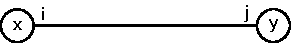
\includegraphics[scale=1]{images/n_14}\\
%           (x e y diventano connessi)
%         \end{center}
%   \item Siccome l'avversario gioca contro le entità, prima di consegnare il
%         messaggio di $x$, sveglia $y$ ed aspetta a consegnare il messaggio.
% \end{itemize}
% In generale, quando $x \in  \xi$ vuole mandare un messaggio, l'avversario guarda
% i link a cui $x$ manda i messaggi e sveglia tutte le entità non ancora sveglie
% (posticipando la consegna dei messaggi).

% Supponiamo $G'$ sia il grafo composto da nodi svegli, consideriamo $G''$
% composto da nodi non svegli isomorfo a $G'$:

% \begin{center}
%   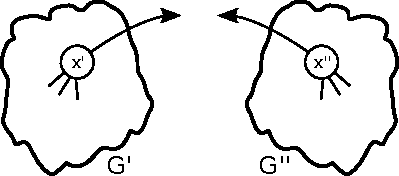
\includegraphics[scale=1]{images/n_15}
% \end{center}

% $G'$ e $G''$ sono sconnessi e sono isomorfi poiché consideriamo grafi completi.

% Quando creiamo il collegamento tra $G'$ e $G''$ diciamo che l'avversario è in un
% \textit{nuovo STAGE}.\\
% Quindi \textbf{STAGE(i)} equivale al momento in cui due sottoinsiemi di entità
% vengano unite dallo scambio reciproco di un messaggio.\\
% \end{comment}
